\setchapterstyle{kao}
\setchapterpreamble[u]{\margintoc}

\chapter{Standard Model Neutrinos and Beyond}
\labch{sm_neutrinos_properties}


\section{The Standard Model}

The \textit{Standard Model (SM)} of particle physics is a Yang-Mills theory \sidecite[1.5cm]{yang_mills} providing very accurate predictions of weak, strong, and \textit{electromagnetic (EM)} interactions. It is a relativistic quantum field theory that relies on gauge invariance, where all matter is made up of fermions, which are divided into quarks and leptons, and bosons describe the interactions between the fermions that have to fulfil the overall symmetry of the theory. Leptons are excitations of Dirac-type fermion fields.

The initial idea of the theory is associated with the works of Weinberg \sidecite{weinberg}, Glashow \sidecite{Glashow}, and Salam \cite{Salam}, that proposed a unified description of EM and weak interactions as a theory of a spontaneously broken SU(2) x U(1) symmetry for leptons, predicting a neutral massive vector boson $Z^0$, a massive charged vector boson $W^\pm$, and a massless photon $\gamma$ as the gauge bosons. The Higgs mechanism \sidecite{higgs}, describing the breaking of the symmetry, predicts the existence of an additional scalar particle, the Higgs boson, giving the $W^\pm$ and $Z^0$ bosons their mass. The Higgs boson was discovered in 2012 at the LHC \sidecite{higgs_discovery_cms, higgs_discovery_atlas}.

Gell-Mann and Zweig proposed the quark model in 1964 \sidecite{gellmann, zweig}, which was completed by the discovery of non-abelian gauge theories \cite{non_abel_gauge} to form the SU(3) symmetry of the strong interaction called \textit{quantum chromodynamics (QCD)}. QDC describes the interaction between quarks and gluons which completed the full picture of the SM in the mid-1970s. Together with the electroweak theory, the SM is a SU(3)$_C$ x SU(2)$_L$ x U(1)$_Y$ local gauge symmetry, with the conserved quantities $C$, \textit{color}, $L$, \textit{left-handed chirality}, and $Y$, \textit{weak hypercharge}

In the following, the basic properties of the SM are described, following the derivations of \sidecite{giunti, schwartz}.


\subsection{Fundamental Fields}

Fermions in the SM are Weyl fields with either \textit{left-handed (LH)} or \textit{right-handed (RH)} chirality, meaning they are eigenvectors of the chirality operator $\gamma_5$ with $\gamma_5 \psi_{R/L}=\pm \psi_{R/L}$. Only LH particles transform under SU(2)$_L$. The Higgs field is a complex scalar field, a doublet of SU(2)$_L$, which is responsible for the spontaneous symmetry breaking of SU(2)$_L$ x U(1)$_Y$ to U(1)$_\rm{EM}$. Local gauge transformations of the fields are given by
\begin{equation}
    \psi \rightarrow e^{i g \theta^a(x) T^a} \psi
    \;,
\end{equation}
where $g$ is the coupling constant, $\theta^a(x)$ are the parameters of the transformation, and $T^a$ are the generators of the group, with $a$ counting them. The number of bosons is dependent on the generators of the symmetry groups, while the strength is defined by the coupling constants. There are eight massless gluons corresponding to the generators of the SU(3)$_C$ group. These mediate the strong force which conserves color charge. The $W_1, W_2, W_3$, and $B$ boson fields of the SU(2)$_L$ x U(1)$_Y$ group are mixed into the massive bosons through spontaneous symmetry breaking as
\begin{equation}
    W^\pm = \frac{1}{\sqrt{2}} (W_1 \mp i W_2)
\end{equation}
and
\begin{equation}
    Z^0 = \cos \theta_W W_3 - \sin \theta_W B
    \;,
\end{equation}
with $\theta_W$ being the \textit{Weinberg angle}. The massless photon field is given by
\begin{equation}
    A = \sin \theta_W W_3 + \cos \theta_W B
\end{equation}
and its conserved quantity is the EM charge $Q$, which depends on the weak hypercharge, $Y$, and the third component of the weak isospin, $T_3$, as $Q = T_3 + Y/2$.

\begin{margintable}
    \footnotesize
    \begin{tabular}{ ccccc }
    \hline\hline    
     & \multicolumn{3}{c}{\textbf{Type}} & \textbf{Q} \\     
    \hline\hline    
    \multirow{2}{*}[-0.3em]{ quarks } & u & c & t & +2/3 \\
    & d & s & b & -1/3 \\
    \hline
    \multirow{2}{*}[-0.3em]{ leptons } & $\nu_e$ & $\nu_{\mu}$ & $\nu_{\tau}$ & 0 \\
     & $e$ & ${\mu}$ & ${\tau}$ & -1 \\
    \hline
    \end{tabular}
\caption[Standard model fermions]{Fermions in the Standard Model. Shown are all three generations of quarks and leptons with their electric charge $Q$.}
\labtab{fermions}
\end{margintable}

Fermions are divided into six quarks and six leptons. Weak, strong, and EM force act on the quarks, and they are always found in bound form as baryons or mesons. Leptons do not participate in the strong interaction and only the electrically charged leptons are massive and are effected by the EM force, while neutrinos are massless and only interact via the weak force. Each charged lepton has an associated neutrino, which it interacts with in \textit{charged-current (CC)} weak interactions, that will be explained in more detail in \refsec{weak_interactions}. The fermions are listed in \reftab{fermions}.


\subsection{Electroweak Symmetry Breaking}

To elaborate the process of spontaneous symmetry breaking through which the gauge bosons of the weak interaction acquire their masses, the Lagrangian of the Higgs field is considered as
\begin{equation}
    \mathcal{L}_\rm{Higgs} = (D_\mu \Phi^\dagger) (D^\mu \Phi) - \lambda \left( \Phi^\dagger \Phi - \frac{v^2}{2} \right) ^2
    \;,
    \labeq{higgs_lagrangian}
\end{equation}
with parameters $\lambda$ and $v$, where $\lambda$ is assumed to be positive. $\Phi$ is the Higgs doublet, which is defined as
\begin{equation}
    \Phi = \binom{\Phi^+}{\Phi^0}
    \;,
    \labeq{higgs_doublet}
\end{equation}
with the charged component $\Phi^+$ and the neutral component $\Phi^0$. The covariant derivative is given by
\begin{equation}
    D_\mu = \partial_\mu - i g_2 \frac{\sigma^i}{2} W^i_\mu - \frac{1}{2} i g_1 B_\mu
    \;,
    \labeq{covariant_derivative}
\end{equation}
with the Pauli matrices $\sigma^i$ and the gauge boson fields $W^i_\mu$ and $B_\mu$ of the SU(2)$_L$ and U(1)$_Y$ groups, respectively. The coupling constants $g_2$ and $g_1$ are the respective coupling constants which are related to the Weinberg angle as $\tan{\theta_W} = \frac{g_1}{g_2}$. The Higgs potential has a non-zero \textit{vacuum expectation value (vev)} at the minimum of the potential at $\Phi^\dagger \Phi = \frac{v^2}{2}$. Since the vacuum is electrically neutral, it can only come from a neutral component of the Higgs doublet as
\begin{equation}
    \Phi_\rm{vev} = \frac{1}{\sqrt{2}} \binom{0}{v}
    \;.
    \labeq{higgs_vev}
\end{equation}


\subsection{Fermion Masses} \labsec{fermion_masses}

The mass term for charged fermions with spin-1/2 is given by
\begin{equation}
    \mathcal{L}_\rm{Dirac} = m (\bar{\Psi}_R \Psi_L - \bar{\Psi}_L \Psi_R)
    \;,
    \labeq{dirac_lagrangian}
\end{equation}
composed of the product of left- and right-handed Weyl spinors $\Psi_{L/R}$. This term is not invariant under SU(2)$_L$ x U(1)$_Y$ gauge transformations, but adding a Yukawa term
\begin{equation}
    \mathcal{L}_\rm{Yukawa} = -Y^e \bar{L}_L \Phi e_R + h.c.
    \;,
    \labeq{up_type_yukawa_lagrangian}
\end{equation}
coupling the fermion fields $e_R$ to the Higgs field $\Phi$, recovers the invariance and gives the fermions their masses. Here, $Y^e$ is the Yukawa coupling constant and $\bar{L}_L$ is the SU(2)$_L$ doublet. With the vev, this results in the mass term for the charged leptons and down-type quarks of $-m_e(\bar{e}_L e_R + \bar{e}_R e_L)$ with $m_e = \frac{Y^e v}{\sqrt{2}}$. With $\tilde{\Phi} = i \sigma_2 \Phi^*$, a similar Yukawa term can be written as $-Y^u \bar{L}_L \tilde{\Phi} u_R + h.c.$, which leads to the masses of the up-type quarks.


\subsection{Leptonic Weak Interactions after Symmetry Breaking} \labsec{weak_interactions}

\begin{marginfigure}
    \centering
    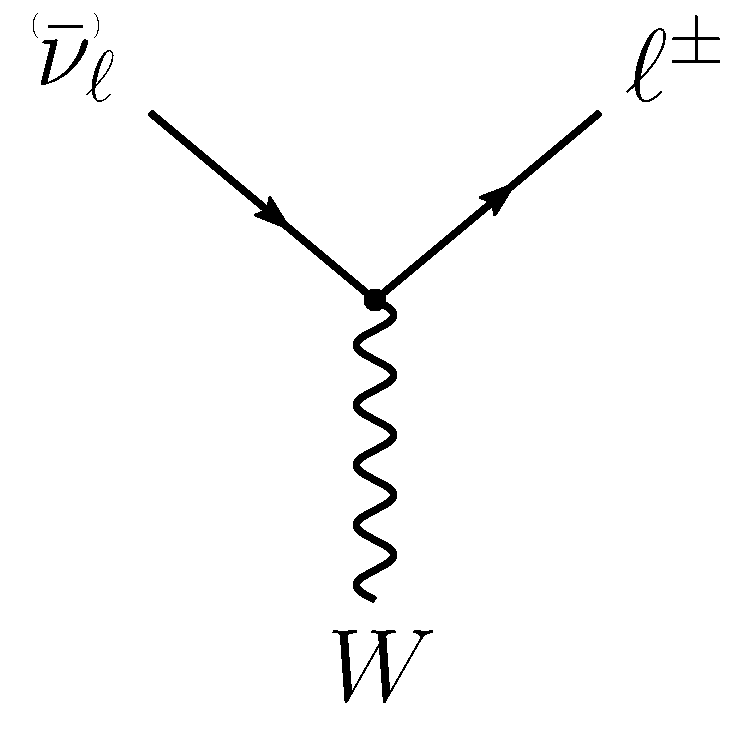
\includegraphics[width=0.49\linewidth]{figures/neutrinos_properties/feynman_CC_nu.pdf}
    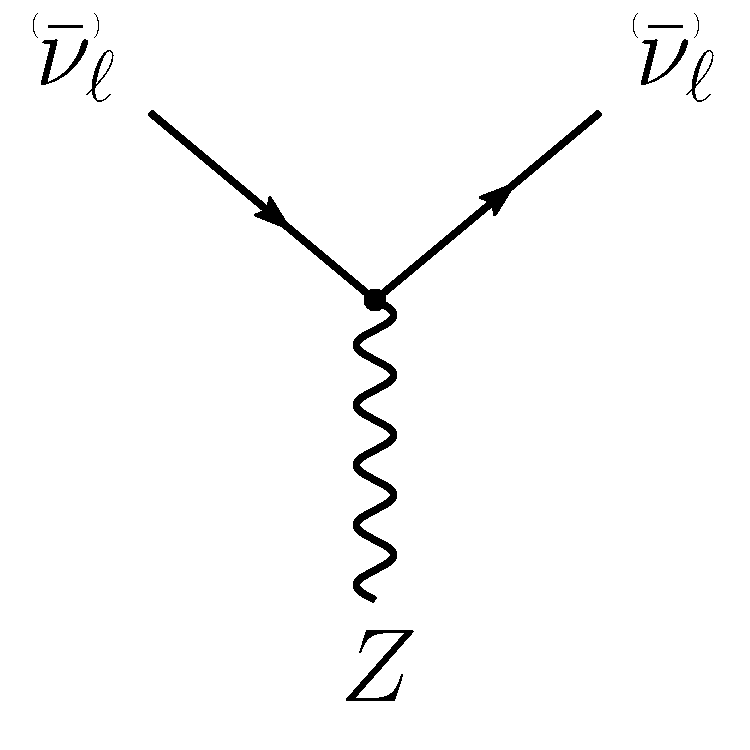
\includegraphics[width=0.49\linewidth]{figures/neutrinos_properties/feynman_NC_nu.pdf}
    \caption[Feynman diagrams of neutrino weak interactions]{Feynman diagrams of charged-current (left) and neutral-current (right) neutrino weak interactions, taken from \cite{ATerliuk}.}
    \labfig{weak_interactions}
\end{marginfigure}    
\todo{Plot is missing + for W and 0 for Z boson. (RED)}

After the spontaneous symmetry breaking, the leptonic part of the electroweak Lagrangian can be written as
\begin{equation}
    \begin{aligned}
        \mathcal{L}^{\ell}_{\rm EW} &= \frac{g}{\sqrt{2}}W^+ \sum _{\alpha=e,\mu,\tau} {\bar{\nu}}_{\alpha}\gamma ^\mu P_L \ell _\alpha + \frac{g}{4c_w} Z \\& \times \left\{ \sum _{\alpha=e,\mu,\tau} {\bar{\nu}}_{\alpha}\gamma ^\mu P_L \nu_{\alpha} + \sum _\alpha {\bar{\ell }}_\alpha \gamma ^\mu \left[ 2s_w^2P_R-(1-2s_w^2)P_L \right] \ell _\alpha \right\} + h.c.
        \;,
    \end{aligned}
    \labeq{extended_leptonic_ew_lagrangian}
\end{equation}
where $c_w \equiv \cos \theta _w$, $s_w \equiv \sin \theta _w$, $P_L$ and $P_R$ are the left and right projectors, respectively, while $\nu_{\alpha}$ and $\ell _\alpha$, are the neutrino and charged lepton weak eigenstates. The $W^+$ and $Z$ bosons are the massive gauge bosons of the weak interaction. The large boson masses $m_{{W}}\sim\SI{80}{\gev}$ and $m_{{Z}}\sim\SI{90}{\gev}$ result in a short range of the force of about \SI{1e-18}{\meter}. Interactions carried out by the ${W}^\pm$ bosons are called \textit{charged current (CC)} interactions, as they propagate a charge, therefore changing the interacting lepton to its charged/neutral counterpart. \textit{Neutral current (NC)} interactions are those mediated by the ${Z}^0$ boson, where no charge is transferred. NC interactions couple neutrinos to neutrinos and charged leptons to charged leptons, but not to each other. The Feynman diagrams for CC and NC interactions are shown in \reffig{weak_interactions}.


\section{Beyond the Standard Model}

The fundamentals of the SM described above \textbf{are not} enough to explain all observed phenomena. Gravity cannot be explained by the SM, as it is incompatible with general relativity, neither can some of the cosmological observations like dark matter, and the matter-antimatter asymmetry be explained. But most importantly, the SM does not predict neutrinos to have mass, which is experimentally proven by neutrino oscillations, so some extension to the SM is needed in order to explain the observed phenomena.

Standard cosmology ($\Lambda$CDM\todo{Cite and/or sidenote this. (RED)}) assumes that equal amounts of matter and anti-matter were produced in the early universe. However, the universe today is dominantly made up of matter. This so-called \textit{baryon asymmetry} can be measured by the difference between the number densities of baryons and anti-baryons normalized to the number density of photons as
\begin{equation}
    \eta_B = \frac{n_B - n_{\bar{B}}}{n_\gamma}
    \;,
\end{equation}
where $n_B$, $n_{\bar{B}}$, and $n_\gamma$ are the number densities of baryons, anti-baryons, and photons, respectively. Baryons are the dominant component with  $\eta_B$ being observed to be around $6 \times 10^{-10}$\todo{cite this (RED)}. Leptogenesis and EW baryogenesis are scenarios that could explain this phenomenon, where the former could be realized by the existence of heavy RH neutrinos.

The observation of neutrino flavor conversions and neutrino oscillations in a multitude of experiments \sidecite{homestake, super_k_atm_osc, snolab_flavor_conv} is the strongest evidence for physics beyond the SM measured in laboratories to date. The observation that neutrinos change their flavor while they propagate through space can only be explained, if at least two neutrinos have a non-zero mass. From those measurements we know the mass differences are very small as compared to the lepton masses, but neither their existence, nor their smallness is predicted by the SM. There are upper limits on the sum of all neutrino masses from cosmological observations at \SI{1.2}{\electronvolt} \sidecite{BOS_nu_masses, planck_nu_mass} and at \SI{0.8}{\electronvolt} from the KATRIN experiment \sidecite{katrin_nu_mass}. Adding RH neutrino states to the theory could explain the origin of the observed non-zero neutrino masses and could be tested for by searching for corresponding signatures in experiments.

\todo{highlight a few more neutrino related open questions, to circle back to related to the HNL searches maybe? (YELLOW)}

% \textbf{Open questions related to neutrinos:}
% \begin{itemize}
%     \item question of neutrino nature, e.g. dirac or majorana?
%     \item absolute mass values? (mass ordering + absolute mass scale)
%     \item is there leptonic cp violation and what is the precise delta\_cp value?
%     \item what are the mixing angle values and is there a flavor principle
%     \item is there additional effects like steriles, non-standard, lorentz violation
% \end{itemize}


\subsection{Mass Mechanisms}

Since there are no RH neutrinos in the SM, the mass mechanism described in \refsec{fermion_masses}, which couples the Higgs field to LH and RH Weyl fields, predicts the LH neutrinos to be massless. From experimental observations it is known that at least two of the three neutrino generations need to have a non-zero mass. Assuming the existence of RH neutrinos fields $\nu_{R}$, one way of producing the neutrino masses is by adding a Yukawa coupling term similar to the one for up-type quarks mentioned in \refsec{fermion_masses}, to write the full Yukawa Lagrangian as
\begin{equation}
    \mathcal{L}_\rm{Yukawa} = -Y^e_{ij} \bar{L}^i_L \Phi e^j_R - Y^\nu_{ij} \bar{L}^i_L \tilde{\Phi} \nu^j_R + h.c.
    \;,
    \labeq{dirac_yukawa_lagrangian}
\end{equation}
with $i,j$ running over the three generations of leptons $e$, $\mu$, and $\tau$, and $Y^e$ and $Y^\nu$ being the Yukawa coupling matrices. Diagonalizing the Yukawa coupling matrices through unitary transformations $U^e$ and $U^\nu$ leads to the \textbf{Dirac mass term} in the mass basis as
\begin{equation}
    \mathcal{L}^\rm{mass}_\rm{Dirac} = \frac{v}{\sqrt{2}} \left( \bar{e}_L M_e e_R - \bar{\nu}_L M_\nu \nu_R \right)
    \;,
    \labeq{dirac_mass_lagrangian}
\end{equation}
where $M_e$ and $M_\nu$ are the diagonal mass matrices of leptons and neutrinos, respectively. A purely Dirac mass term would not explain the smallness of the neutrino masses in a straightforward way. Only fine-tuning the Yukawa coupling constants to small values would lead to small neutrino masses.

An additional way of generating neutrino masses is by adding a Majorana mass term of the form
\begin{equation}
    \mathcal{L}_\rm{Majorana} = -\frac{1}{2} M_{ij} (\nu^i_R)^c \nu^j_R + h.c.
    \;,
    \labeq{majorana_mass_lagrangian}
\end{equation}
with $M_{ij}$ being the Majorana mass matrix and the indices $i, j$ running over all $n_R$ RH neutrino generations. The superscript $c$ denotes the charge conjugate field. Combining the charge conjugated RH neutrino fields with the LH neutrino fields as
\begin{equation}
    \boldsymbol{N} = \binom{\boldsymbol{\nu}_L}{\boldsymbol{\nu}_R^c}
    \;,
\end{equation}
with $\boldsymbol{\nu}_R$ containing the $n_R$ RH fields. The full neutrino mass Lagrangian is then given by the combined \textbf{Dirac and Majorana mass term} as
\begin{equation}
    \mathcal{L}^\rm{mass, \nu}_\rm{Dirac+Majorana} = \frac{1}{2} \boldsymbol{N}^T \hat{C} M^\rm{D+M} \boldsymbol{N} + h.c.
    \;,
    \labeq{dirac_and_Majorana_mass_lagrangian}
\end{equation}
and the mass matrix is given by
\begin{equation}
    M^\rm{D+M} = \begin{pmatrix}
    0 & (M^D)^T \\
    M^D & M^R
    \end{pmatrix}
    \;.
    \labeq{dirac_and_Majorana_mass_matrix}
\end{equation}
On top of explaining the origin of neutrino masses itself, a combined Dirac and Majorana mass term could also solve the question of their smallness. If the mass of the RH neutrinos is very large, the masses of the active neutrino flavors is suppressed, which is known as \textit{see-saw mechanism}.



minimal scenario needed to explain the two observed non-zero SM neutrino masses is two RH neutrinos

mixing between mass and flavor eigenstates is then described by a 5x5 mixing matrix

\todo{I need to esplain the SM PMNS matrix before this, otherwise I'm missing that here.. (RED)}



\subsection{Observational Avenues for Right-Handed Neutrinos}

if the RH neutrinos have masses at the eV scale, they can be observed through variations in neutrino oscillation experiments as was done in OscNext and MEWOWs analysis in IceCube \todo{cite these and add some more (RED)} and they could explain the observed anomalies in xyz (take some info from Alex), cite alex thesis for a more thorough overview?

heavy RH neutrinos, also known as heavy neutral leptons, are too massive to be produced in oscillations and would have to be searched for in direct production and decay experiments that will be discussed in more detail in the following


\subsection{Searching for Heavy Neutral Leptons} \labsec{HNL_mixing_constraints}


\subsubsection{Colliders}

LHC: proton-proton collider
sqrt(s): 7, 8, 13


ATLAS/CMS: nearly hermetic detectors around interaction, multiple searches for HNL scenarios
LHCB: forward detector, designed to search for new particles in decays of heavy hadrons

Type I Seesaw Results:

HNL production in GeV reange from : decays of heavy mesons, tau leptons, W bosons, H bosons, or top quarks
HNL decays: to lepton number conserving (dirac), or lepton number conserving and violating channels (majorana), depending on mass and mixing parameters, prompt and displaced decays are possible


Atlas results set constraints on mixing with e and mu:

Atlas in minimal extension: ~$10^-6$ with \um4 at 4-10 GeV
same for CMS: ~$10^-5$ with \um4 and \ue4 at 10-600 GeV

CMS: final state of 3 leptons (two opposite charged and nu) giving \um4 ~$4*10^-7$ at 8-14 GeV

the above mentioned (strong) constraints are mostly based on a model with one HNl coupling to one flavor
in type 1 seesaw at least 2 are needed to see the two SM nu masses, both coupling to several flavors
it was shown (cite) that re-interpreting these results with more than one HNL can lead to much weaker constraints and to compare results, the assumed model and couplings have to be considered
the strong reduction in constraints is due to the opening of new channels, to which the search may not be sensitive

more complex scenarios are possible and might produce various signatures, but are harder to measure: extended gauge symmetries, effective field theories

type III seesaw (HNL as SM EW triplets) can be observed as they are produced in pairs (no active-sterile mixing needed) and result in multi lepton states and high pt jets -> strong exclusion of masses below 790 GeV


LHCb: low mass and high mass results (above below mW), competitive in low mass

low mass channel: B+ -> mu+ N -> pi+ mu-, at order ~$10^-3$ for \um4 at 0.5-3.5 GeV

high mass channel: W+ -> mu+ mu+-jet, at order $10^-3$-$10^-2$ / $10^-4$-$10^-3$ for \um4 at 5-50 GeV for LNC/LNV


there is a shit ton of future colliders and/or experiments at the LHC planned, that have sensitivities to HNLs.. think about which/how to discuss them


\subsubsection{Nuclear Decay}

novel approach to search for HNLs through energy-momentum conservation measurements in nuclear reactions

mixing of HNL with electon nu/nubar would cause irregularities, interpretable as limits in \ue4 and m4


\paragraph{Beta Decay}

detect kinks in the energy spectra at $Q-m_4c^2$

m4 probable between energy detection threshold and Q value of the decay

tritium 3H: Q=18.6 keV

planned analysis in KATRIN and TRISTAN (1 to 18 keV mass) projected statistical upper limits (95) around $10^-7$ \ue4 (but will need detector upgrades)

in Project 8 measure the absolute neutrino mass using cyclotron radiation emission spectroscopy (CRES), may also be able to search for HNLs


atmospheric argon 39Ar: Q=565keV

DUNE: massive LArTPCs at long baseline (1300km) accelerator nu (1GeV), measure ionization charge of 39Ar beta decays: projected sensitivity in 20kev to 450keV mass range for \ue4 at $10^-7$ (requires substantial trigger development), without more like $10^-5$


\paragraph{Electron Capture}

requires total energy-momentum reconstruction of non nu final states in electron capture

e capture: pure 2-body decay of recoiling atom and electron neutrino (mono energetic)
measureing atom and associated de-excitation xray or auger electron, energy momentum conservation can be probed

separated non-zero missing mass peak would indicate HNL mixing with the electron neutrino/antineutrino

BeEST experiment: 100-850 keV mass, 7Be (Q=862keV), previous results at $10^-4$ \ue4, future sensitivity at $10^-7$ \ue4 after upgrades to the experiment

(proposed) HUNTER experiment: 20-300 keV mass (K-capture of 131Cs), "significantly improve current limits"


\paragraph{Reactor Searches}

MeV masses (up to 12) at short baseline reactor experiments (commercial or research reactors)

source of electron antineutrinos, therefore also HNL (if they mix)

visible channels: N to nu e+ e-, and N to nu gamma, nu gamma gamma, where the first dominates

pioneering analysis reports $10^-4$ \ue4 at 2-7 MeV mass range


many experiments exist at 5-25 meters from reactor core, at 100 MW research or 1 GW commercial reactors and 1-5 m3 volume detectors.. these are designed to adress reactor anomaly, but could most likely also proble decay in flight to electron positron


\subsubsection{Extracted Beamlines}

protons interacting with a target or a beam dumb can produce pions, kaons, and heavy-quark hadrons, which can decay to neutrinos and HNLs

HNLs from those interactions can have energies of 1 MeV to 5 GeV and decay at long distances, because of their long lifetimes (model dependent)

experiments using a spectrometer with particle identification can detect unique decay signatures at displaced vertices

the observable signature is just a displaced vertex from for example N to l pi, N to l+ l-, N to nu pi0 etc., which cannot be explained by SM neutrinos, without scattering process (not sufficient mass)

depending on the decay channel, a specific mixing can be probed

the other way of searching for HNLs with this is to look for peaks in the missing mass spectrum at the production vertex (at target)

HNL search pioneer work was done by experiments at extracted beam lines, with early results from PS191, CHARM, NOMAD reporting bounds from direct production and decay of HNLs

today there is a large activity of searches for HNLs at extracted beamlines and the strongest bounds on decays are by recent results at PIENU [24, 25], NA62 [28, 29], T2K [36, 514], MicroBooNE [515, 516], and ArgoNeuT [517] experiments

as a standard, the results are presented with only one non-zero mixing parameter at a time

show strongest limits for all three mixings?


\begin{figure}
  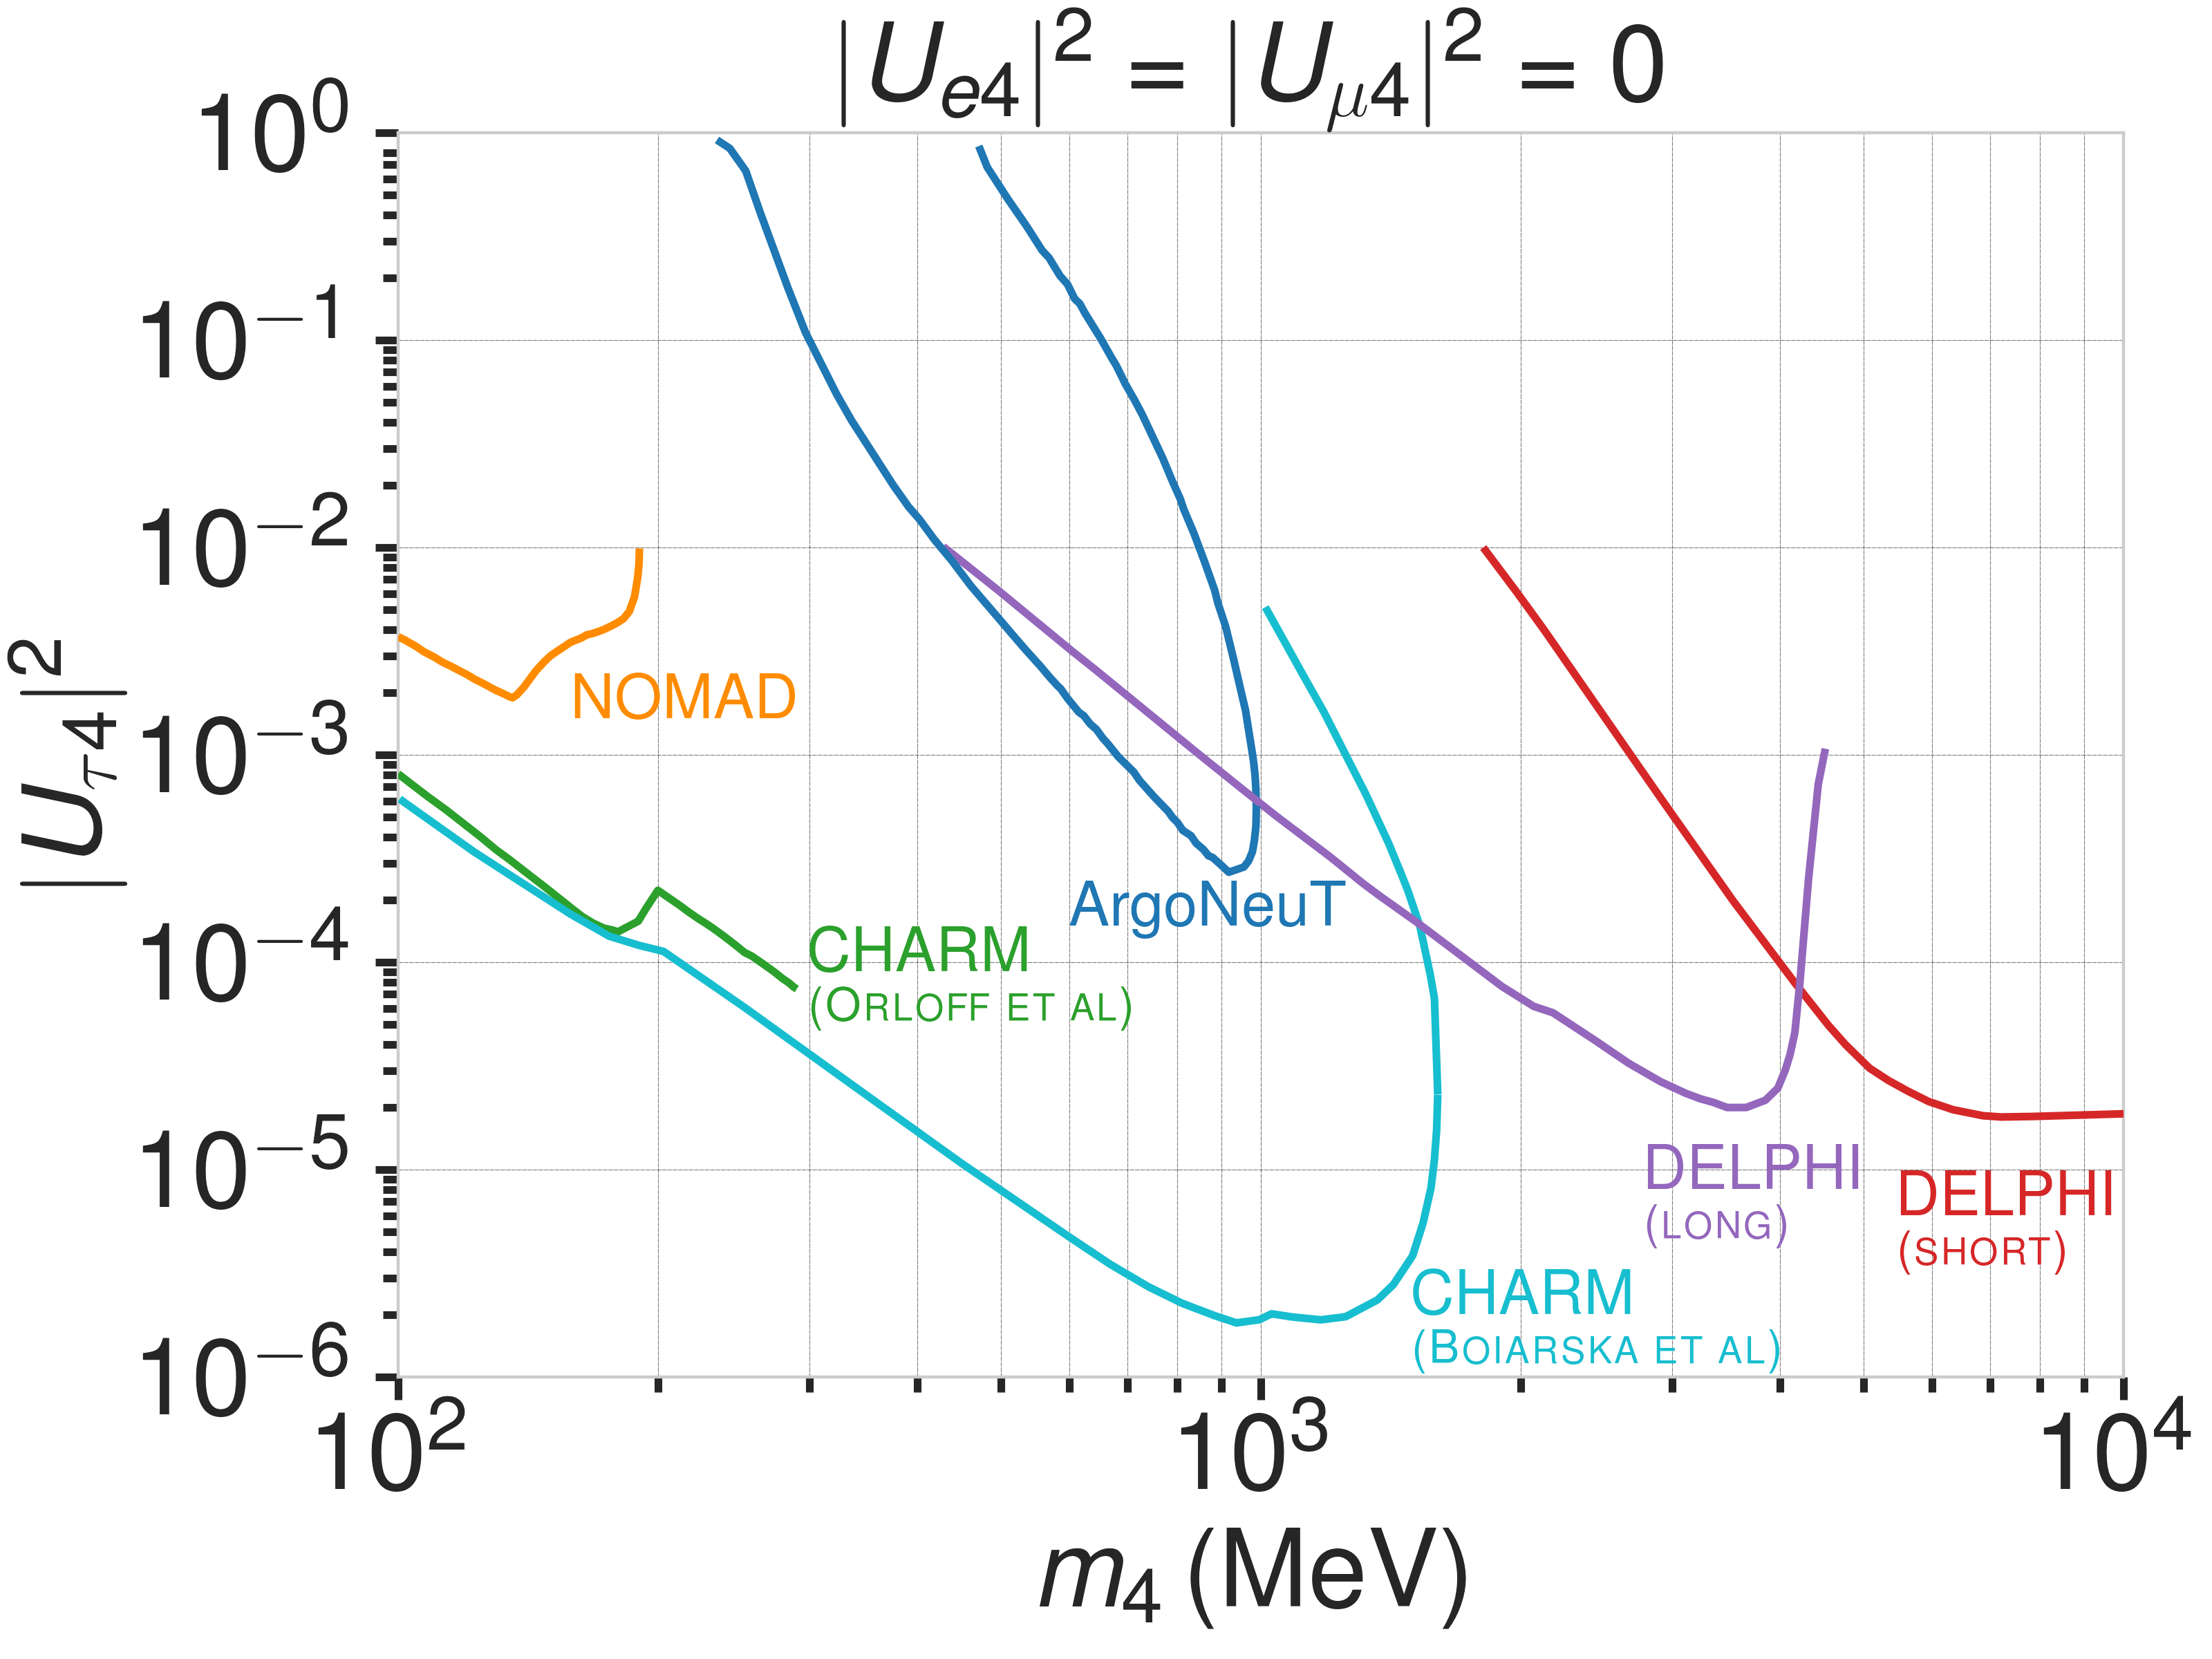
\includegraphics{figures/hnl_simulation/theory/UtauN_custom_plots_LF_grid_white.png}
  \caption[Current $|U_{\tau4}^2|-m_4$ limits]{Current $|U_{\tau4}^2|-m_4$ limits from NOMAD \cite{NOMAD:2001eyx}, ArgoNeut \cite{ArgoNeuT:2021clc}, CHARM \cite{Orloff:2002de, Boiarska:2021yho}, and DELPHI \cite{DELPHI:1996qcc}.}
  \labfig{boundsUtau}
\end{figure}


\subsubsection{Atmospheric and Solar}

natural sources of neutrinos up to 20 MeV (solar) and 100s of GeV (atmospheric)

both provide all flavors because of mixing/oscillations and can therefore be used to probe mixing with $nu_e$, $nu_mu$, and $nu_tau$

depending on the mass and mixing, which govern the decay length, different signatures can be used to probe large parts of the phase space

depending on the type of coupling (just mass-mixing, or more complicated like dipole-portal) considered, the scales could be different


\paragraph{Production in the Sun}

if the HNL lifetimes are large enough, they could reach the detector after being produced in the sun

this will only allow production through non-zero \ue4 and not the other mixings

measurements of the decay to e+ e- nu and comparing to the expected inter-plenatry positron flux as was done in Borexino lead to the strongest limits in the few MeV regime

KAMLAND and Super-K could potentially also search for this through the inverse beta decay


\paragraph{Upscatter outside of the Detector}

for HNL decay length scales of the order of the Earth's diameter, the HNLs could be upscattered anywhere in the earth from the solar or atmospheric neutrino fluxes and decay in the detector

for masses below 18 MeV, limits were derived in [37] R. Plestid (2020), 2010.04193 and [585] R. Plestid (2020), 2010.09523 (just tau-coupled for mixing and all flavor for dipole-portal) and decay in Borexino

in principle this could also be possible for atmospheric neutrinos, but flux and oscillation have to be taken into account

direct production of HNLs in the atmosphere is also possible, but has not been investigated yet

\paragraph{Production and Decay in the Detector}

If HNL decay lengths are sufficiently short, production and decay could happen in the detector and the observation of two vertices could be used to constrain the mixing parameters

in principle mixing with any neutrino flavor produced in the sun or the atmosphere could be probed and theoretical studies have been performed for mass-mixing and dipole-portal couplings for IceCube and Super-K, Hyper-K, Dune

expand a bit more, or just jump to my section?


\subsubsection{Cosmological and Astrophysical}

leave these out for the moment?


\section{Atmospheric Neutrinos as Source of Heavy Neutral Leptons} \labsec{hnl_theory}


\subsection{Production of Neutrinos in the Atmosphere}

The analysis performed in this work is based on the sample of neutrinos observed in IceCube DeepCore at energies below \SI{100}{\gev}. At these energies, the flux exclusively originates in the Earth's atmosphere. Highly relativistic cosmic rays (protons and heavier nuclei \sidecite{PhysRevD.98.030001}) interact in the upper atmosphere, producing showers of secondary particles. Neutrinos are produced in decays of charged pions and kaons ($\pi$ and $K$ mesons) present in those showers, where the dominant contribution comes from the decay chain
\begin{equation}
    \begin{split}   
        \pi^\pm &\rightarrow \mu^\pm + \nu_\mu(\bar{\nu}_\mu)\;, \\
        \mu^\pm &\rightarrow e^\pm + \bar{\nu}_\mu(\nu_\mu) + \nu_e(\bar{\nu}_e)
        \;,
    \end{split}
    \labeq{pion_decay}
\end{equation}
where muon neutrinos $\nu_\mu$ and muons $\mu^\pm$ are produced in the first decay and both electron and muon neutrinos $\nu_{e/\mu}$ are produced in the second decay. Atmospheric muons, which are also produced in these decays, are the main background component for IceCube DeepCore analyses.

\begin{figure}
    \centering
    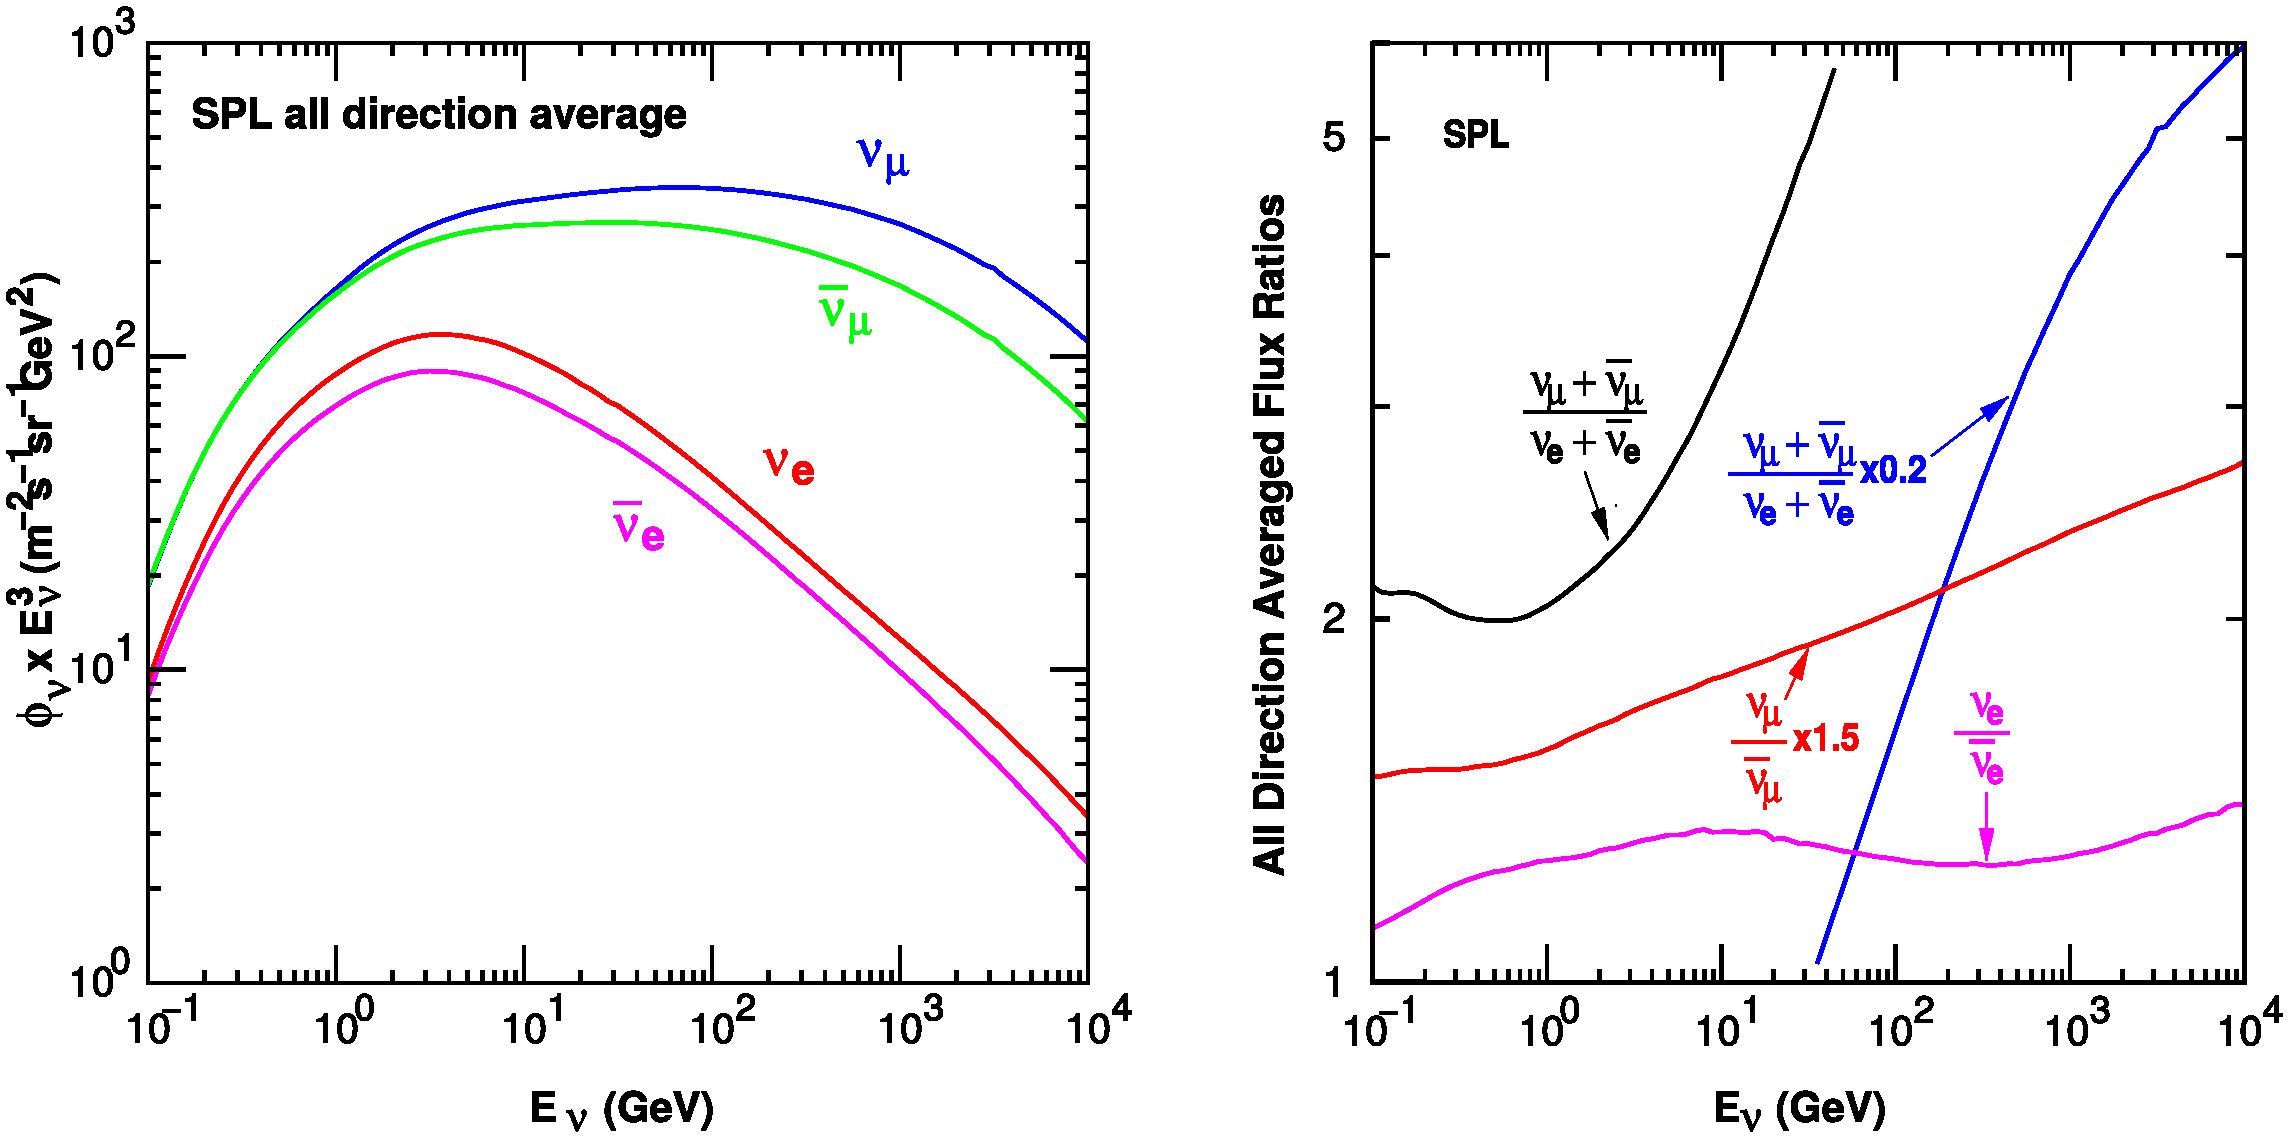
\includegraphics[width=1.0\textwidth]{figures/neutrinos_properties/Honda_alldir-spl_copy.pdf}
    \caption[Atmospheric neutrino fluxes]{The atmospheric fluxes of different neutrino flavors as a function of energy (left) and the ratios between muon neutrinos and electron neutrinos as well as the ratios between neutrinos and antineutrinos for both those flavors (right). Results from the calculations performed for the geographic South Pole, taken from \cite{PhysRevD.92.023004_Honda_Flux}.}
    \labfig{honda_flux}
\end{figure}

The different atmospheric flux components are shown in \reffig{honda_flux} (left), for a much broader energy range than relevant for this work. Both neutrinos and antineutrino fluxes are shown for electron  and muon neutrinos and all fluxes are the directionally averaged expectation calculated at the South Pole. Muon neutrinos are dominating the flux and from \refeq{pion_decay} the naive assumption would be that the ratio between muon and electron neutrinos is $(\nu_\mu+\bar{\nu}_\mu)/(\nu_e+\bar{\nu}_e)=2$. This is roughly true at energies below \SI{1}{\gev}, where all muons decay in flight, but at larger energies muons can reach the detector before decaying, which increases the ratio to approximately 10:1 at around \SI{100}{\gev}. Additionally, kaon decays start to contribute which also increases the number of muons and muon neutrinos. The increasing ratio can be seen in \reffig{honda_flux} (right), which also shows the ration between neutrinos and antineutrinos for both flavors.

Charged mesons or tau particles can also be produced in cosmic ray interactions. Their decays lead to the production of tau neutrinos. At the energies relevant for this work however, the resulting tau neutrino flux is negligible as compared to the muon neutrino flux \sidecite{2015EPJWC..9908001F_lepton_fluxes} and is not considered in the analysis. This is because both charged mesons and tau particles are much heavier than pions and kaons and therefore their production is suppressed at high energies.\todo{Say something about atmospheric neutrino flux uncertainties, based on recent JP/Anatoli papers. (YELLOW)}
% It should be stated here that there is a rather large uncertainty on the normalization of the atmospheric neutrino flux on the order of 20-30\,\% \sidecite{PhysRevD.75.043006_neutino_flux_honda} in the energy region of interest.
% This is mainly due to uncertainties in the primary cosmic ray spectrum and modeling of the hadronic interactions.\todo{SB:
% I don't think this is true - the normalization is known to ~5\% if you trust Anatoli/Juan Pablo. Please have a look at more recent publications on this topic.}


\subsection{Oscillations} \labsec{neutrino_oscillations}

So far we have described neutrinos in their flavor eigenstates, which are relevant for weak interactions. In the SM three-neutrino model the weak flavor states are $\nu_e, \nu_\mu$, and $\nu_\tau$, which relate them to the charged leptons they interact with in CC interactions. There is a second way of describing neutrino wave functions based on their Hamiltonian eigenvalues \sidecite{BILENKY1978225}, namely as the mass eigenstates $\nu_1, \nu_2$, and $\nu_3$. These states are related to the flavor eigenstates by the unitary, 3x3 \textit{Pontecorvo-Maki-Nakagawa-Sakata (PMNS)} matrix $U$, where the flavor states are a superposition of the mass states as
\begin{equation}
    \ket{\nu_\alpha} = \sum_kU^*_{\alpha k}\ket{\nu_k}
    \;,
    \labeq{neutrino_mixing}
\end{equation}
with the weak flavor states $\ket{\nu_\alpha}$, $\alpha=e,\mu,\tau$, and the mass states $\ket{\nu_k}$ with $k=1,2,3$. The mixing matrix can be parameterized as \sidecite{PhysRevD.98.030001}
\begin{equation}
    U=\left( 
    \begin{matrix}
        1 & 0 & 0 \\
        0 & c_{23}  & s_{23} \\
        0 & -s_{23} & c_{23} 
    \end{matrix}
    \right) 
    \left( 
    \begin{matrix}
        c_{13} & 0 & s_{13}e^{-i\delta_{CP}} \\
        0 & 1 & 0\\
        -s_{13} e^{i\delta_{CP}} & 0 & c_{13}
    \end{matrix}
    \right) 
    \left( 
    \begin{matrix}
        c_{12} & s_{12} & 0 \\
        -s_{12} & c_{12} & 0\\
        0 & 0 & 1
    \end{matrix} 
    \right)  
    \;,
    \labeq{PMNS_matrix}
\end{equation}
where $c_{ij}=\cos\theta_{ij}$ and $s_{ij}=\sin\theta_{ij}$ are cosine and sine of the mixing angle $\theta_{ij}$, that defines the strength of the mixing between the mass eigenstates $i$ and $j$, and $\delta_{CP}$ is the neutrino CP-violating phase.\todo{add current BF values from nufit or so? (YELLOW)}

Describing neutrinos in their mass state is crucial to understand their propagation through space and time. Their propagation in vacuum can be expressed by applying a plane wave approach, where the mass eigenstates evolve as
\begin{equation}
    \ket{\nu_k(t)} = e^{-iE_kt/\hbar}\ket{\nu_k}
    \;.
    \labeq{flavor_time_evol}
\end{equation}
The energy of the mass eigenstate $\ket{\nu_k}$ is $E_k=\sqrt{\vec{p}^2c^2+m_k^2c^4}$, with momentum $\vec{p}$ and mass $m_k$, $\hbar$ is the reduced Planck constant, and c is the speed of light in vacuum. The existence of non-zero, non-equal masses and the neutrino mixing relation in \refeq{neutrino_mixing}, lead to the observed phenomenon of neutrino oscillations. Oscillations mean that a neutrino changes from its initial flavor, that it was produced with, to another flavor and back after traveling a certain distance. A neutrino is produced as a flavor eigenstate $\ket{\nu_\alpha}$ in a CC weak interaction, but its propagation happens as the individual mass states it is composed of. The probability of finding the neutrino with initial flavor $\ket{\nu_\alpha}$ in the flavor state $\ket{\nu_\beta}$ after the time $t$ is calculated as
\begin{equation}
    P_{\nu_\alpha \rightarrow \nu_\beta}(t)
    =
    |\braket{\nu_\beta|\nu_\alpha(t)}|^2
    \;,
    \labeq{fermis_golden_rule}
\end{equation}
by applying Fermi's Golden Rule \sidecite{1927RSPSA.114..243D}, which defines the transition rate from one eigenstate to another by the strength of the coupling between them. This coupling strength is the square of the matrix element and using the fact that the mixing matrix is unitary ($U^{-1}=U^\dagger$) to describe the mass eigenstates as flavor eigenstates, we find the time evolution of the flavor state $\ket{\nu_\alpha(t)}$, which can be inserted into \refeq{fermis_golden_rule} to find the probability as
\begin{equation}
    P_{\nu_\alpha \rightarrow \nu_\beta}(t)
    =
    \sum_{j,k}U^*_{\beta j}U_{\alpha j}U_{\beta k}U^*_{\alpha k}e^{-i(E_k-E_j)t/\hbar}
    \;.
    \labeq{probability_raw}
\end{equation}
The indices $j$ and $k$ run over the mass eigenstates. We can approximate the energy as
\begin{equation}
    E_k \approx E+\frac{c^4m^2_k}{2E} \hspace{0.25cm} \longrightarrow \hspace{0.25cm} E_k-E_j \approx \frac{c^4\Delta m^2_{kj}}{2E}
    \;,
\end{equation}
for small neutrino masses compared to their kinetic energy. Here, $\Delta m^2_{kj}=m^2_k-m^2_j$ is the mass-squared splitting between states $k$ and $j$. Replacing the time in \refeq{probability_raw} by the distance traveled by relativistic neutrinos $t\approx L/c$ we get
\begin{equation}
    \begin{split}
        P_{\nu_\alpha \rightarrow \nu_\beta}(t)
        = 
        \delta_{\alpha \beta}
        -
        4\sum_{j>k}&\textbf{Re}(U^*_{\beta j}U_{\alpha j}U_{\beta k}U^*_{\alpha k})\textrm{sin}^2\Big( \frac{c^3\Delta m^2_{kj}}{4E\hbar}L \Big) \\
        +
        2\sum_{j>k}&\textbf{Im}(U^*_{\beta j}U_{\alpha j}U_{\beta k}U^*_{\alpha k})\textrm{sin}^2\Big( \frac{c^3\Delta m^2_{kj}}{4E\hbar}L \Big)
        \;,
    \end{split}
    \labeq{probability_detailed}
\end{equation}
which is called the survival probability if $\alpha=\beta$, and the transition probability if $\alpha\neq\beta$. Once again, this probability is only non-zero if there are neutrino mass eigenstates with masses greater than zero. Additionally, there must be a mass-squared difference $\Delta m^2$ and non-zero mixing between the states. Since we assumed propagation in vacuum in \refeq{flavor_time_evol}, the transition and survival probabilities correspond to vacuum mixing. \todo{say something about how this changes with matter (YELLOW)}


\subsection{Interactions with Nuclei} \labsec{neutrino_interactions}

The neutrino detection principle of IceCube DeepCore is explained in \refch{icecube} and relies on the weak interaction processes between neutrinos and the nuclei of the Antarctic glacial ice. At neutrino energies above \SI{5}{\gev}, the cross-sections are dominated by \textbf{\textit{deep inelastic scattering (DIS)}}, where the neutrino is energetic enough to resolve the underlying structure of the nucleons and interact with one of the composing quarks individually. As a result the nucleon breaks and a shower of hadronic secondary particles is produced. Depending on the type of interaction, the neutrino either remains in the final state for NC interactions or is converted into its charged lepton counterpart for CC interactions. The CC DIS interactions have the form
\begin{equation}
    \begin{split}
        \nu_l + N \rightarrow l^- + X \;, \\
        \bar{\nu}_l + N \rightarrow l^+ + X \;, \\
    \end{split}
    \labeq{dis_cc}
\end{equation}
where $\nu_l$/$\bar{\nu}_l$ and $l^-$/$l^+$ are the neutrino/antineutrino and its corresponding lepton/antilepton, and $l$ can be either an electron, muon, or tau. $N$ is the nucleon and $X$ stands for any set of final state hadrons. The NC DIS interactions are
\begin{equation}
    \begin{split}
    \nu_l + N & \rightarrow \nu_l + X \; \rm{and} \\
    \bar{\nu_l} + N & \rightarrow \bar{\nu_l} + X \;.
    \end{split}
    \labeq{dis_nc}
\end{equation}
\reffig{dis_feynman} shows the Feynman diagrams for both processes
\begin{figure}[h]
    \centering
    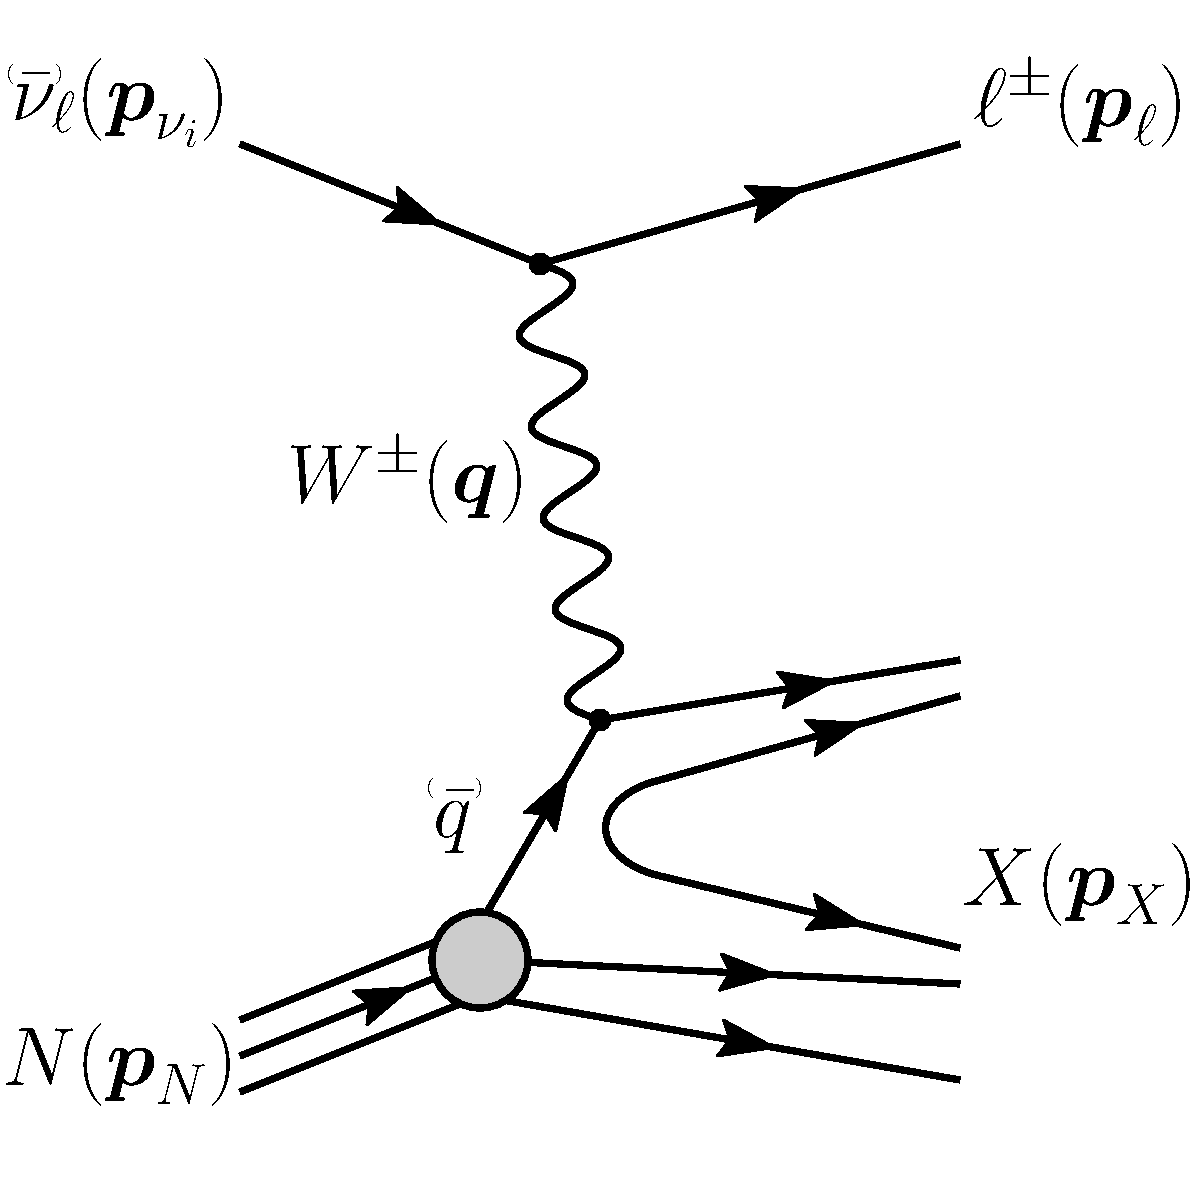
\includegraphics[width=0.4\linewidth]{figures/neutrinos_properties/feynman_DIS_CC_nu_new.pdf}
    \hspace{0.8cm}
    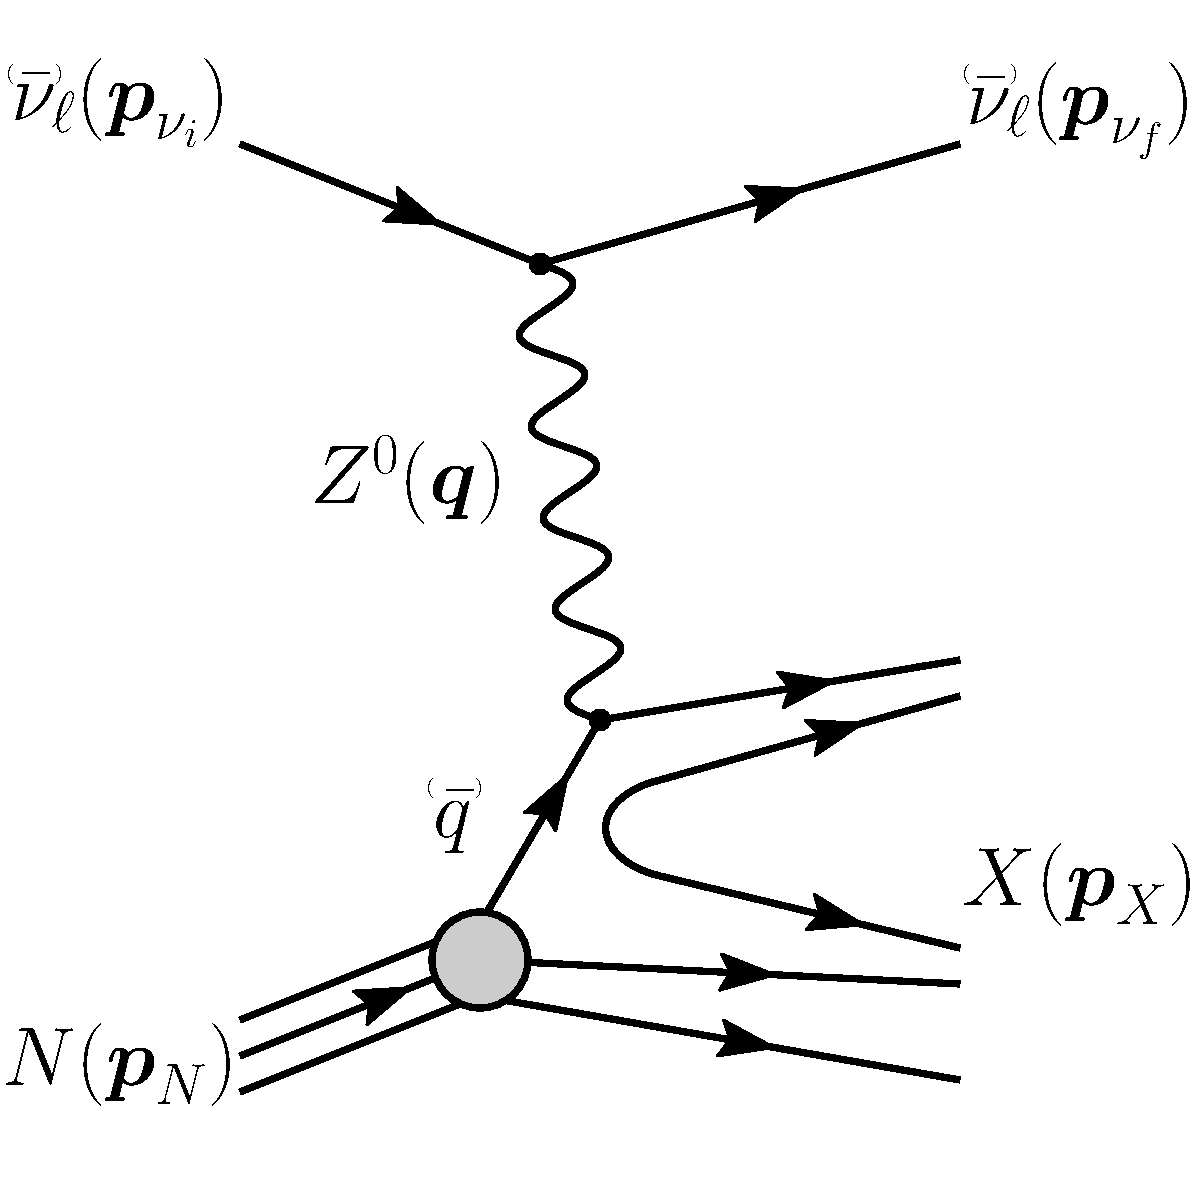
\includegraphics[width=0.4\linewidth]{figures/neutrinos_properties/feynman_DIS_NC_nu_new.pdf}
    \caption[Neutrino-nucleon deep inelastic scattering]{Feynman diagrams for deep inelastic scattering of a neutrino with a nucleon via charged-current (left) and neutral current (right) interactions. $\boldsymbol{p}_{\nu_i}$, $\boldsymbol{p}_{N}$ and $\boldsymbol{p}_{\nu_f}$, $\boldsymbol{p}_{l}$, $\boldsymbol{p}_{N}$ are the input and output four-momenta, while $\boldsymbol{q}$ is the momentum transfer. Taken from \cite{ATerliuk}.}
    \labfig{dis_feynman}
\end{figure}
DIS interactions have a roughly linear energy dependent cross-section above $\sim$\SI{20}{\gev} and are well measured and easy to theoretically calculate. They are the primary interaction channel for neutrinos detected with IceCube.

At energies below \SI{5}{\gev}, \textbf{\textit{quasi-elastic scattering (QE)}} and \textbf{\textit{resonant scattering (RES)}} become important. At these energies the neutrinos interact with the approximately point-like nucleons, without breaking them up in the process. RES describes the process of a neutrino scattering off a nucleon producing an excited state of the nucleon in addition to a charged lepton. It is the dominant process at \SIrange{1.5}{5}{\gev} for neutrinos and \SIrange{1.5}{8}{\gev} for antineutrinos. Below \SI{1.5}{\gev} QE is the main process, where protons are converted to neutrons in antineutrino interactions and vice-versa for neutrino interactions. Additionally, a charged lepton corresponding to the neutrino/antineutrino flavor is produced. The cross-sections of QE and RES scattering processes are not linear in energy and the transition region from QE/RES to DIS is poorly understood. The total cross-sections and their composition is shown in \reffig{neutrino_cross_sections}. It can be seen that the interaction cross-sections are very small at the order of $10^{-38}\mathrm{\,cm}^2$. This is the reason why very large volume detectors are required to measure atmospheric neutrinos with sufficient statistics to perform precision measurements of their properties. The interaction length of a neutrino with $E_\nu = \SI{10}{\gev}$ is of $\mathcal{O}(\SI{10e10}{\kilo\meter})$, for example.

\begin{figure*}[h]
	\centering
    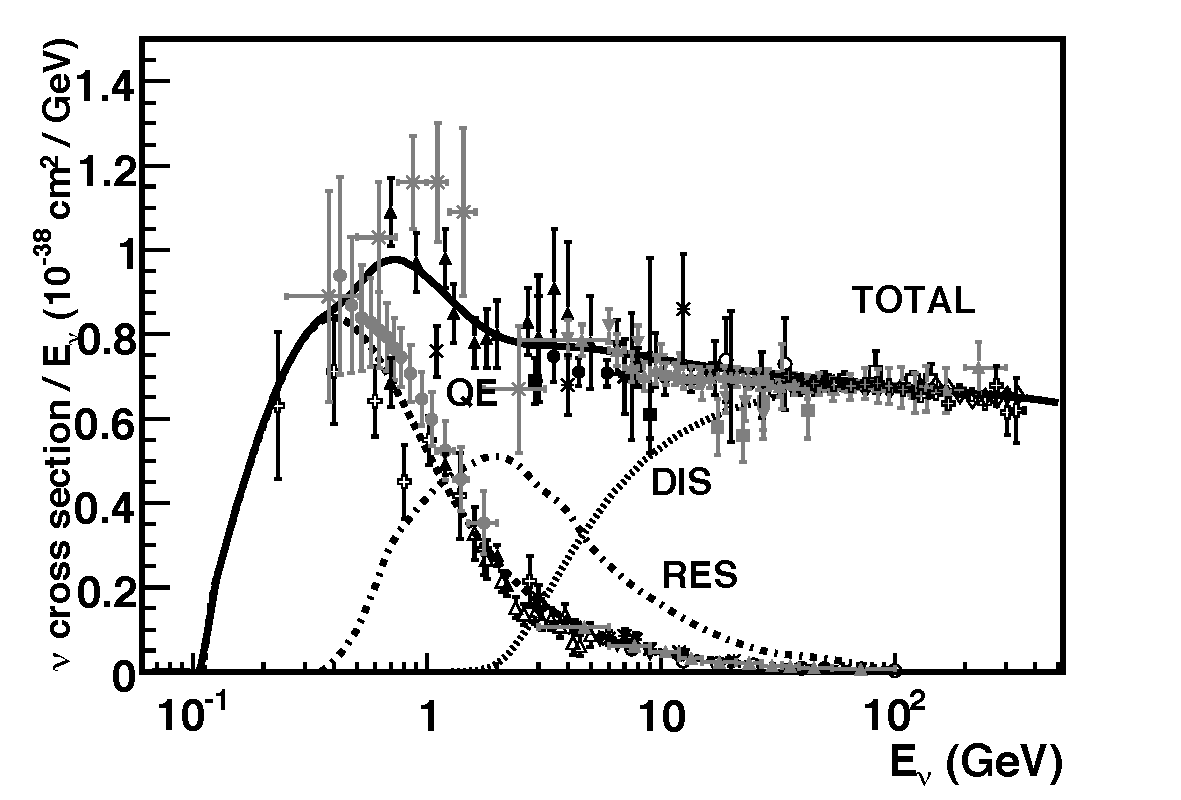
\includegraphics[width=0.495\linewidth]{figures/neutrinos_properties/cc_inclusive_nu.pdf}
    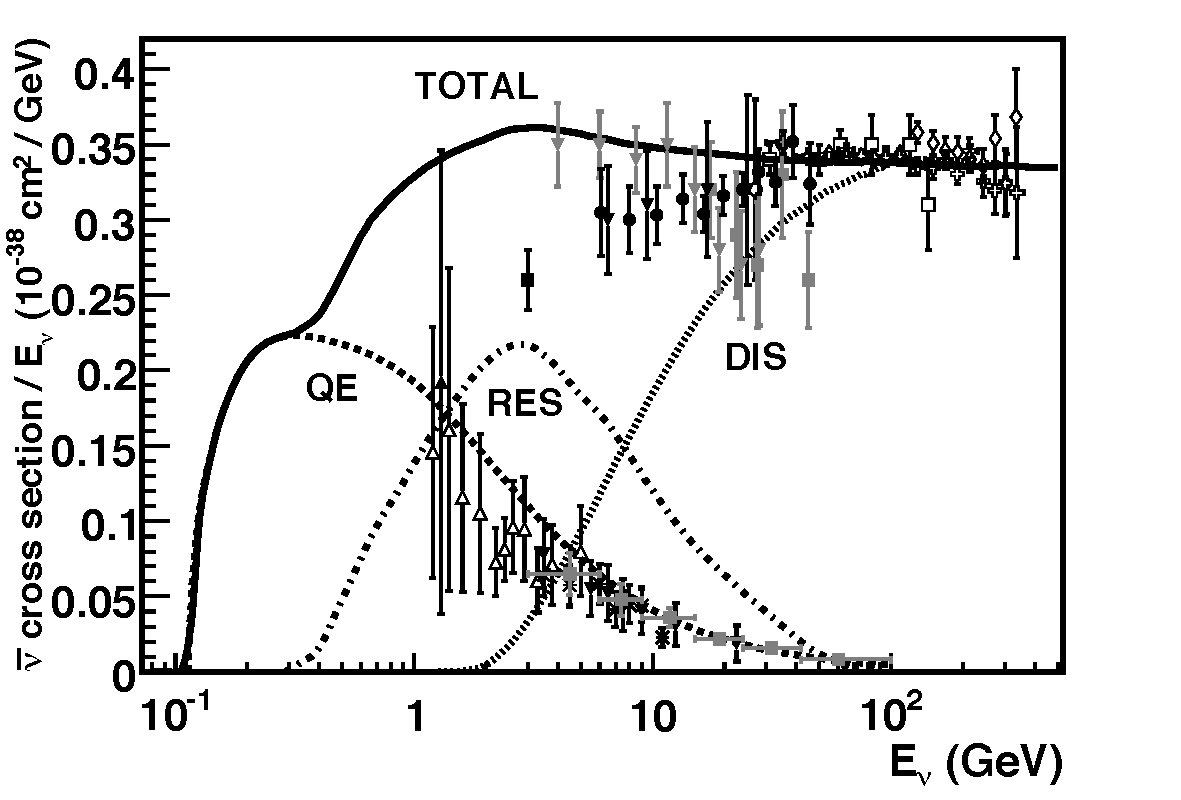
\includegraphics[width=0.495\linewidth]{figures/neutrinos_properties/cc_inclusive_nubar.pdf}
	\caption[Total inclusive neutrino-nucleon cross-sections]{Total neutrino (left) and antineutrino (right) per nucleon cross-section divided by neutrino energy plotted against energy.
    The three main scattering processes quasi-elastic scattering (QE), resonant scattering (RES), and deep-inelastic scattering (DIS) are shown. Taken from \cite{Formaggio_Cross_Sections}.}
    \labfig{neutrino_cross_sections}
\end{figure*}


\subsubsection{HNL Production and Decay} \labsec{double_cascade_morphology}


\paragraph{Up-Scattering in the Ice}


\paragraph{Decay in the Ice}


\begin{figure}
    \includegraphics{figures/hnl_simulation/decay_theory/hnl_decay_widths_up_to_1.0_GeV_log.png}
    \caption[HNL decay widths]{Decay widths of the HNL within the mass range considered, calculated based on the results from \cite{Coloma:2020lgy}. Given the existing constraints on $|U_{e4}|^{2}$ and $|U_{\mu4}|^{2}$, we consider that the corresponding decay modes are negligible.}
    \labfig{hnl_decay_modes_log_decay_width}
\end{figure}


\todo{Re-write/re-formulate this section (copied from HNL technote). (RED)}

% Extensions to the Standard Model (SM) that add \textit{Heavy Neutral Leptons (HNLs)} provide a good explanation for the origin of neutrino masses through different seesaw mechanisms \sidecite{PTP.64.1103}.
% \begin{figure}
%   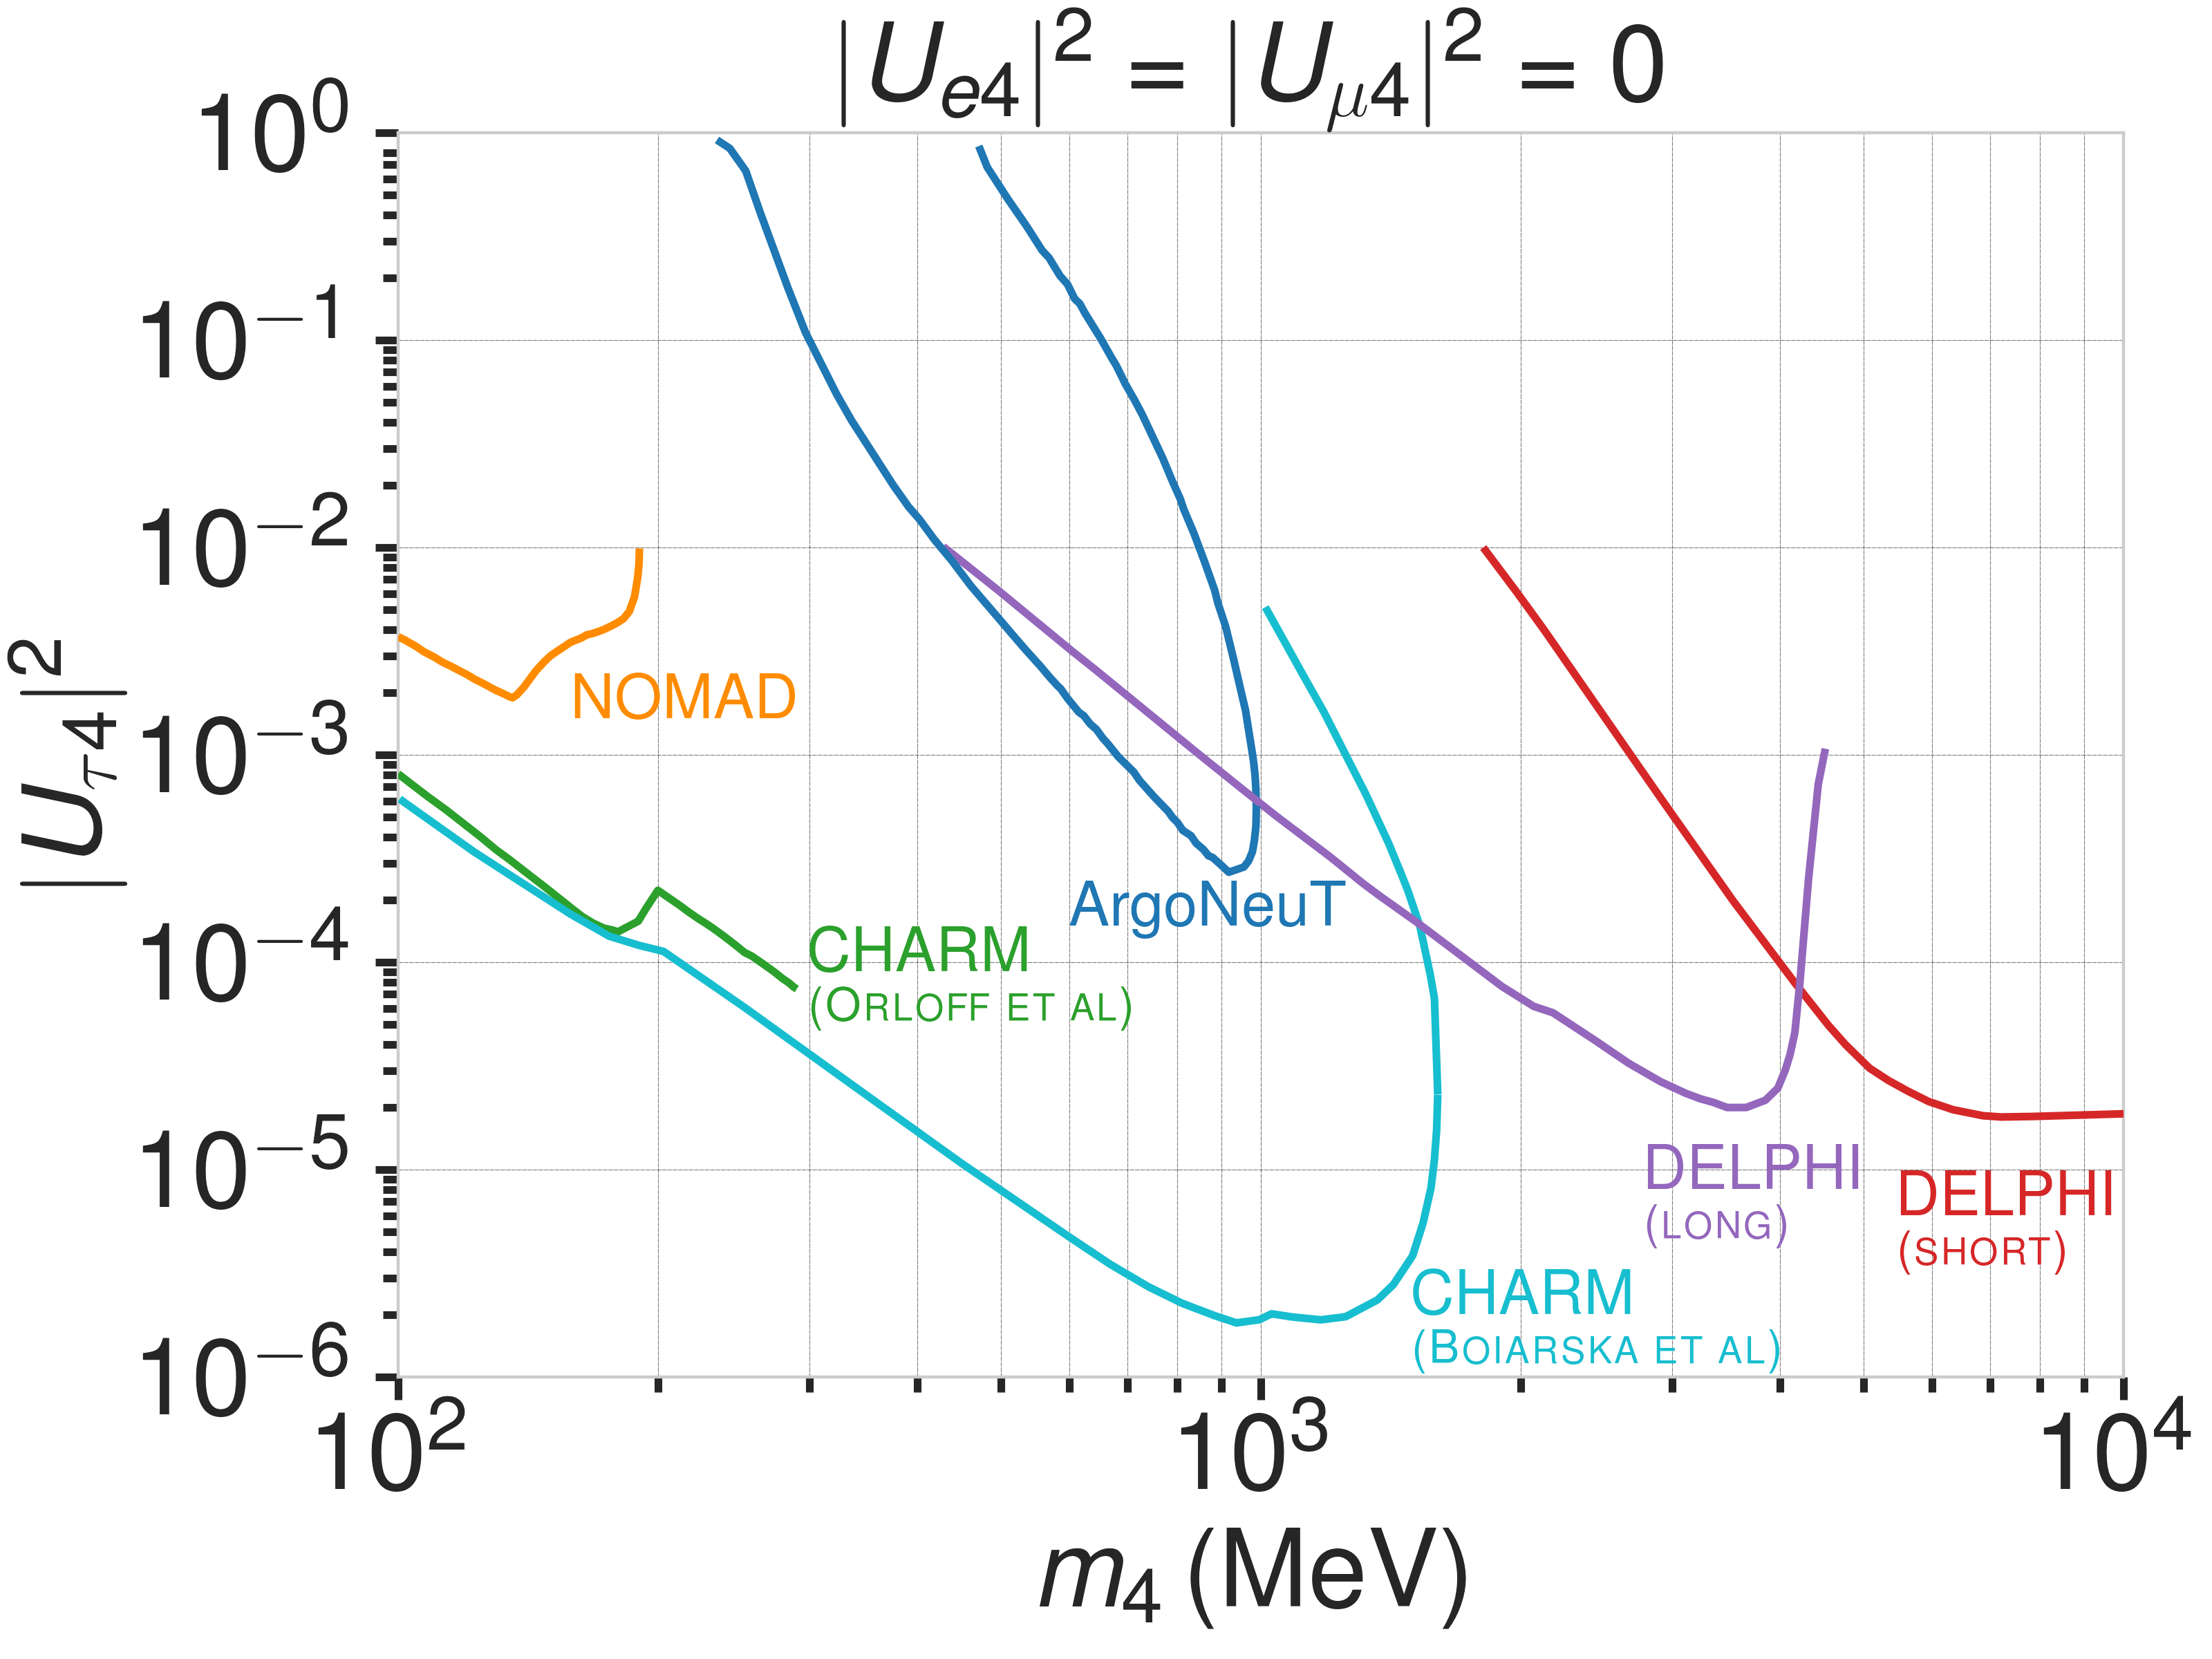
\includegraphics{figures/hnl_simulation/theory/UtauN_custom_plots_LF_grid_white.png}
%   \caption[Current $|U_{\tau4}^2|-m_4$ limits]{Current $|U_{\tau4}^2|-m_4$ limits from NOMAD \cite{NOMAD:2001eyx}, ArgoNeut \cite{ArgoNeuT:2021clc}, CHARM \cite{Orloff:2002de, Boiarska:2021yho}, and DELPHI \cite{DELPHI:1996qcc}.}
%   \labfig{boundsUtau}
% \end{figure}
% While the mixing with $\nu_{e/\mu}$ is strongly constrained\todo{Produce similar styled plot for these limits} ($|U_{\alpha4}^2| \lesssim 10^{-5}-10^{-8}, \alpha=e,\mu$), the mixing with $\nu_{\tau}$ is much harder to probe due to the difficulty of producing and detecting $\nu_\tau$. \reffig{boundsUtau} shows the current limits on the $\tau$-sterile mixing space for HNL masses between $0.1$\,GeV-$10$\,GeV. As was first pointed out in \sidecite{Coloma:2017ppo}, the atmospheric neutrino flux observed in IceCube offers a way to constrain the neutrino-HNL mixing parameters. By using the large fraction of atmospheric $\nu_{\mu}$ events that oscillate into $\nu_{\tau}$ before they reach the detector, the less constrained $\tau$-sterile mixing space can be explored. In this document, we present the methodology and strategy of a search for HNLs with IceCube DeepCore. These additional RH neutrinos can be included in the Standard Model (SM) by extending the PMNS matrix to at least a 3x4 matrix as
% \begin{equation}
%     \begin{pmatrix}
%     \nu_{e}\\
%     \nu_{\mu}\\
%     \nu_{\tau}\\
%     \nu_{s}\\
%     \end{pmatrix}
%     =
%     \begin{pmatrix}
%     U_{e1} & U_{e2} & U_{e3} & U_{e4}\\
%     U_{\mu1} & U_{\mu2} & U_{\mu3} & U_{\mu4}\\
%     U_{\tau1} & U_{\tau2} & U_{\tau3} & U_{\tau4}\\
%     U_{s1} & U_{s2} & U_{s3} & U_{s4}\\
%     \end{pmatrix}
%     \begin{pmatrix}
%     \nu_{1}\\
%     \nu_{2}\\
%     \nu_{3}\\
%     \nu_{4}\\
%     \end{pmatrix}
%     \;,
%     \labeq{4_by_4_mixing_matrix}
% \end{equation}
% where the components with index $4$ define the mixing between the flavor states and the fourth sterile mass state, respectively. Note here that this is not a theoretically fully consistent picture, but rather the phenomenologically minimal model to be tested by this analysis. This can hopefully be put into the larger context of several fully consistent models, later. Due to the singlet nature of the RH neutrinos, they only interact weakly, inheriting these interactions from their LH neutrino counterparts via mixing. This mixing of the HNLs with the electron, muon, and tau neutrinos can be probed and constrained as a function of the HNL mass by searching for their production and decay. In \sidecite{Coloma:2017ppo, Coloma:2019qqj} this search is mainly motivated through two experimental arguments\todo{This section really needs to be re-written to motivate the search for HNLs from a more generic point of view (e.g. to explain neutrino masses)}.
% % First, a decaying sterile neutrino could explain the low-energy excess (LEE) that is observed in the MiniBooNE data \sidecite{PhysRevLett.110.161801}.
% Secondly, IceCube is ideally placed to explore the yet unconstrained $|U_{\tau4}|^{2}-m_{4}$ phase-space that is not easily accessible by accelerator-based experiments.


% In order to probe the $\tau$-sterile mixing parameter, it is required to look at interactions involving $\tau$ neutrinos. However, most neutrinos produced in cosmic ray interactions with the atmosphere are $\nu_{e}$ or $\nu_{\mu}$. Therefore, we need these neutrinos to oscillate to the $\tau$ flavor before reaching the detector. For this to happen at the considered energies a traveled distance of the order of the earth diameter is necessary. This is why our signal is mostly up-going and passing through the whole earth.\todo{This section definitley needs to be elaborated in a little more detail}

To explain the signature we can observe in IceCube we first have to revisit the weak interactions that the HNL inherits from its LH counterpart through mixing. We will be following the derivation in \sidecite{Coloma:2020lgy}. Extending the SM by n additional RH neutrinos, $\nu_i$ ($i=3+n$), leads to the mass Lagrangian
\begin{equation}
    \mathcal{L}_{\nu }^{\rm mass} \supset - \sum _{\alpha = e,\mu ,\tau} \sum _{i=4}^{3+n} Y_{\nu , \alpha i} {\overline{L}}_{L,\alpha} {\tilde{\phi }} \nu_{i} - \frac{1}{2} \sum _{i=4}^{3+n} M_{i} {\overline{\nu}}_{i} \nu^c_{i} + h.c.,
    \labeq{hnl_mass_lagrangian}
\end{equation}
in a basis where the Majorana mass terms are diagonal. $Y_{\nu , \alpha i}$ are the Yukawa couplings to the lepton doublets and $M$ the Majorana masses for the heavy singlets. $L_{L,\alpha}$ stands for the SM LH lepton doublet of flavor $\alpha$ while $\phi$ is the Higgs field, and ${\tilde{\phi }} = i \sigma _2 \phi ^*$ and $\nu^c_{i} \equiv C {\bar{\nu}}_{i}^t$, with $C = i \gamma _0 \gamma _2$ in the Weyl representation. The full neutrino mass matrix with the Higgs vacuum expectation value $v/\sqrt{2}$ reads
\begin{equation}
    {\mathcal {M}} = \left( \begin{array}{cc} {\mathbf {0}}_{3\times 3} &{} Y_\nu v/\sqrt{2} \\ Y_\nu ^t v/\sqrt{2} &{} M \end{array} \right),
    \labeq{majorana_mass_matrix}
\end{equation}
and can be diagonalized by a $(3+n)$ x $(3+n)$ full unitary roation $U$, that itself leads to neutrino masses upon diagonalization, additionally manifesting the mixing between active neutrinos and heavy states. The resulting model consists of 3 light SM neutrino mass eigenstates $\nu_i$ ($i=1,2,3$) and n heavier states, as introduced above. The flavor states will now consist of a combination of light and heavy states
\begin{equation}
    \nu _\alpha = \sum _{i=1}^{3+n} U_{\alpha i} \nu_i,
    \label{equ:extend_neutrin_flavor_mass_relation}
\end{equation}
and the leptonic part of the EW Lagrangian can be written as
\begin{equation}
    \begin{aligned}
        \mathcal{L}^{\ell}_{\rm EW} &= \frac{g}{\sqrt{2}}W^+_\mu \sum _{\alpha } \sum _{i} U_{\alpha i}^* {\bar{\nu}}_{i}\gamma ^\mu P_L \ell _\alpha + \frac{g}{4c_w} Z_\mu \\& \times \left\{ \sum _{i, j} C_{ij} {\bar{\nu}}_{i}\gamma ^\mu P_L \nu_j + \sum _\alpha {\bar{\ell }}_\alpha \gamma ^\mu \left[ 2s_w^2P_R\!-\!(1\!-\!2s_w^2)P_L \right] \ell _\alpha \right\} + h.c.,
    \end{aligned}
    \labeq{leptonic_ew_lagrangian}
\end{equation}
% where $c_w \equiv \cos \theta _w$, $s_w \equiv \sin \theta _w$, $P_L$ and $P_R$ are the left and right projectors, respectively, while $\nu_{\alpha}$ and $\ell _\alpha$, are the neutrino and charged lepton weak eigenstates
while
\begin{equation}
    C_{ij} \equiv \sum _\alpha U^*_{\alpha i} U_{\alpha j}.
    \labeq{general_squared_mixing}
\end{equation}
The indices now sum over all $(3+n)$ flavor and mass states.

Based on this formulation and assuming that only the mixing with the tau sector is open ($|U_{\alpha4}^2|=0, \alpha=e,\mu$), the relevant production diagram of the HNL can be drawn as shown in \reffig{HNL_production}. Alongside the fourth heavy mass state, a Hadronic cascade is produced. The heavy mass state will travel for some distance (dependent on mass and mixing) before it decays. The subsequent decay processes are depicted in \reffig{HNL_decay}. It can be a CC or NC decay and both leptonic and mesonic modes are possible (dependent on the mass). This will produce a tau or a tau neutrino and another cascade that can be EM or Hadronic. The branching ratios corresponding to the decay modes of the HNL for the mass range of interest (i.e. between \SI{100}{\mev} and 1\,GeV) are shown in \reffig{hnl_decay_modes_log_branching_ratio} as a function of the HNL mass.

% \begin{figure}[!htb]
%     % \footnotesize
%     \centering
%     \begin{fmffile}{figures/feynman_diagrams/diag_HNL_production}
%         \begin{fmfgraph*}(210,70)
%         \fmfleft{i1,i2}
%         \fmfright{o1,o2}
%         \fmf{fermion,label=$q$,label.side=right}{i1,v1,o1}
%         \fmf{fermion,label=$\nu_{\tau}$,label.side=left}{i2,v2}
%         \fmf{fermion,label=$\nu_{4}$,label.side=left}{v2,o2}
%         \fmf{photon,label=$Z$}{v1,v2}
%         \fmflabel{$|U_{\tau 4}|^2$}{v2}
%         \end{fmfgraph*}
%     \end{fmffile}
%     \caption[Feynman diagram of HNL up-scattering process]{Production of a sterile neutrino in the up-scattering of a tau neutrino.}
%     \labfig{HNL_production}
% \end{figure}

% \begin{figure}[!htb]
%     % \footnotesize
%     \centering
%     \begin{fmffile}{figures/feynman_diagrams/diag_HNL_decay_NC}
%         \begin{fmfgraph*}(175,70)
%         %\fmfstraight
%         \fmfleft{i}
%         \fmfright{o1,o2,o3}
%         \fmf{fermion,tension=3.,label=$\nu_{4}$,label.side=left}{i,v1}
%         \fmfv{label=$|U_{\tau 4}|^2$,label.angle=90}{v1}
%         \fmf{fermion,label=$\nu_{\tau}$,label.side=left}{v1,o3}
%         \fmf{photon,tension=3,label=$Z$,label.side=right}{v1,v2}
%         \fmf{fermion,tension=3,label=$f/q/q$,label.side=left}{v2,o2}
%         \fmf{fermion,tension=3,label=$\bar{f}/\bar{q}/\bar{q'}$,label.side=left}{o1,v2}
%         \end{fmfgraph*}
%         \end{fmffile}
%         \begin{fmffile}{figures/feynman_diagrams/diag_HNL_decay_CC}
%         \begin{fmfgraph*}(175,70)
%         %\fmfstraight
%         \fmfleft{i}
%         \fmfright{o1,o2,o3}
%         \fmf{fermion,tension=3.,label=$\nu_{4}$,label.side=left}{i,v1}
%         \fmfv{label=$|U_{\tau 4}|^2$,label.angle=90}{v1}
%         \fmf{fermion,label=$\tau$,label.side=left}{v1,o3}
%         \fmf{photon,tension=3,label=$W$,label.side=right}{v1,v2}
%         \fmf{fermion,tension=3,label=$f/q$,label.side=left}{v2,o2}
%         \fmf{fermion,tension=3,label=$\bar{f'}/\bar{q'}$,label.side=left}{o1,v2}
%         \end{fmfgraph*}
%     \end{fmffile}
%     \caption[Feynman diagram of HNL decay]{Sterile neutrino decay through neutral current (left) and charged current (right).}
%     \labfig{HNL_decay}
% \end{figure}

% \begin{figure}[h]
%     \subfloat[\labfig{hnl_decay_modes_log_branching_ratio}]{
%         \includegraphics[width=.45\linewidth]{figures/hnl_simulation/decay_theory/branching_ratios_log_up_to_1.0_GeV.png}
%     }
%     \subfloat[\labfig{hnl_decay_modes_log_decay_width}]{
%         \includegraphics[width=.45\linewidth]{figures/hnl_simulation/decay_theory/hnl_decay_widths_up_to_1.0_GeV_log.png}
%     }
%     \\[-2.5ex]
%     \centering
%     \subfloat[\labfig{hnl_decay_modes_log_proper_lifetime}]{
%         \includegraphics[width=.45\linewidth]{figures/hnl_simulation/decay_theory/proper_lifetimes_up_to_1.0_GeV_log.png}
%     }
%     \caption[HNL branching ratios]{Branching ratios, decay widths, and proper lifetime of the HNL within the mass range considered, calculated based on the results from \cite{Coloma:2020lgy}.}
%     \labfig{hnl_decay_modes_log}
% \end{figure}


% \paragraph{Potentially useful referecnes}
% \begin{itemize}
%     \item two FeynRules [arXiv:1310.1921] models that have been made publicly
%     available (see ancillary files) so that not only the total branching ratios can be computed,
%     but also differential event distributions can be easily simulated by interfacing the output
%     of FeynRules with event generators such as MadGraph5 [arXiv:1405.0301]
% \end{itemize}


% taken from technote
% \begin{figure}[h]
%     \subfloat[\labfig{hnl_decay_modes_log_branching_ratio}]{
%         \includegraphics[width=.45\linewidth]{hnl_simulation/decay_theory/branching_ratios_log_up_to_1.0_GeV.png}
%     }
%     \subfloat[\labfig{hnl_decay_modes_log_decay_width}]{
%         \includegraphics[width=.45\linewidth]{hnl_simulation/decay_theory/hnl_decay_widths_up_to_1.0_GeV_log.png}
%     }
%     \\[-2.5ex]
%     \centering
%     \subfloat[\labfig{hnl_decay_modes_log_proper_lifetime}]{
%         \includegraphics[width=.45\linewidth]{hnl_simulation/decay_theory/proper_lifetimes_up_to_1.0_GeV_log.png}
%     }
%     \caption{Branching ratios, decay widths, and proper lifetime of the HNL within the mass range considered, calculated based on the results from \sidecite{Coloma:2020lgy}. Given the existing constraints on $|U_{e4}|^{2}$ and $|U_{\mu4}|^{2}$, we consider that the corresponding decay modes are negligible.}
%     \labfig{hnl_decay_modes_log}
% \end{figure}
